\vspace{-0.3cm}\section{INTRODUCTION}
With the fast development of Internet, image search and recommendation play an important role in delivering information in our daily life. In these applications, measuring the distance (or similarity) of pair-wise images is a fundamental and important issue. \emph{If an effective image distance metric is obtained, we can easily employ existing technologies to achieve satisfactory performance in image search \cite{visualrank} and recommendation \cite{cbf}.}

However, to date, existing image distance metrics do not perform well to achieve this goal, due to the fact that they usually focus on measuring similarity of visual features but are not mature to capture human cognition, which is one of the most important factors in image search and recommendation. Here human cognition includes many aspects, such as semantics, attributes, user intention, image emotion, etc. Although the problem of capturing human cognition has received increasing attention in recent years, how to identify users' cognition is still a great challenge because we can hardly obtain the knowledge.

 With the development of social network, a huge amount of users share their beautiful pictures and view others' in the social media platforms, such as Flickr and Twitter. Within these platforms, we can obtain not only vast amounts of images but also a series of collective social and behavioral information, such as annotated tags, favorite images and interest groups of users. In social psychology, it has been proved that human cognition and user behavior influence each other \cite{cognitive}. Therefore, social behavioral information in social media platform can be regarded as the reflection of their cognition to images. Given user behavior information in the social media platforms, we can use to better evaluate image distance. However, this idea faces the following challenges:


 %Although the technologies up to date can hardly estimate the user cognition behind his behavior, we can easily evaluate the similarity of user behaviors of two images. For a pair of images, if users have similar behaviors (such as favoring, sharing and tagging), their cognition to the images would also be similar. In this paper, we refer to the similarity of users' social behaviors as social similarity.



(1) \textbf{The lack of social information in Web image.} Although behavioral information does help to estimate user cognition, most of the Web images do not have user behavior information due to the fact that they are not produced by social media platforms. If the image distance relies on  social behavioral data, our method will be extremely circumscribed in social images. Therefore, how to make our distance metric universal in common Web images is a great challenge in our problem.

(2) \textbf{The unreliability of social media data.} In social network, collective social and behavioral information is usually uncertain and unreliable. If the amount of user behavior information is not enough, the social similarity may have contingency. For example, although two images are both favored by a user, they may be still dissimilar because the user might have more than one interest. Thus, we also need to consider the reliability of social similarity.

(3) \textbf{The sparsity of user behavior.} In traditional image distance learning task, the knowledge of similarity graph is very dense: in most cases, the similarity of any two images is
fixed. However, in social network, most of pair-wise images are not related socially. Thus, we cannot determine whether these two images are socially similar or not. In this case, the visual similarity should be maintained.
%(3) The Heterogeneity of social data. Different with traditional homogeneous data structure, the data in social media is heterogeneous  and hybrid. For example, a user may publish and favor a lot of images and an image may be shared to a series of interest groups. Therefore, to make our method extensible, we should formulate these multi-modal information in a unified structure.

\begin{figure*}
\label{framework}
\centering
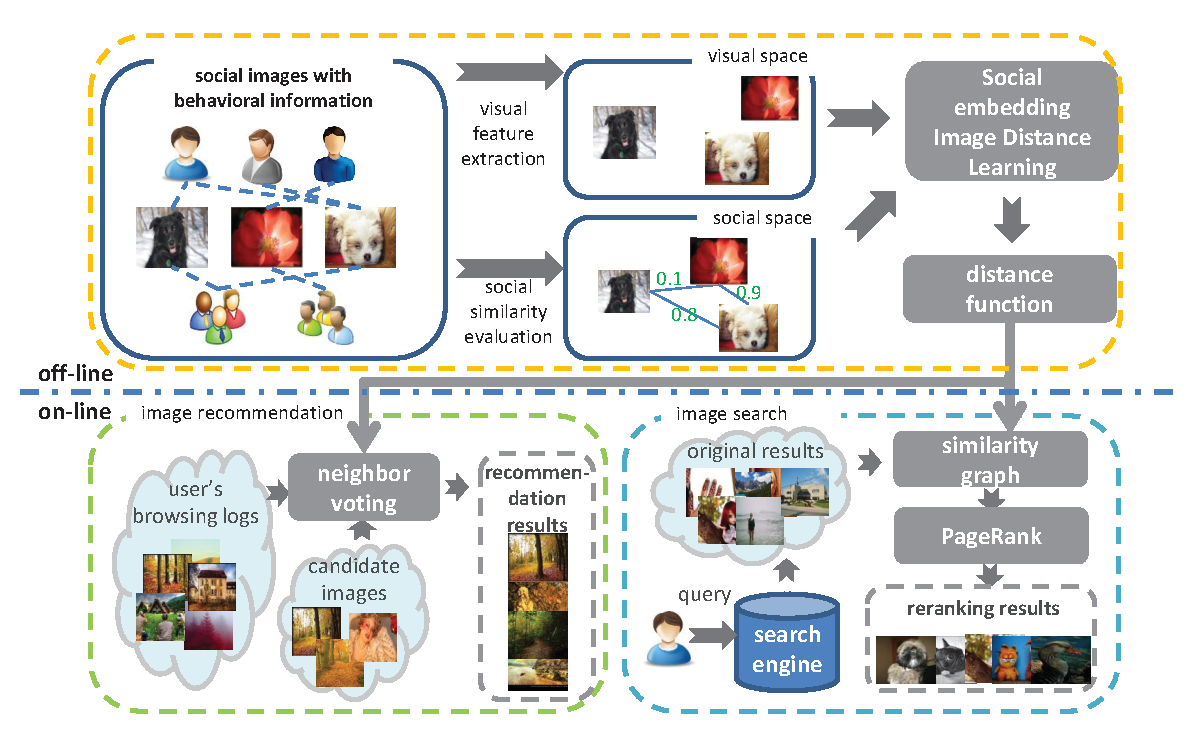
\epsfig{file=framework.eps, width = 5.2in, height = 2.4in}
\caption{Illustration of the proposed Social embedding Image Distance Learning (\emph{SIDL}) approach and the image search and recommendation system developed on \emph{SIDL}.}
\vspace{-0.4cm}
\end{figure*}

To address the above problems, we propose a Social embedding Image Distance Learning (\emph{SIDL}) approach to learn image distance from user behavior information in social media platforms, which is shown in Figure \ref{framework}. In the approach, we use metric learning technique to learn an image distance function of visual features. Different from traditional metric learning work, our distance function aims at making image distance consistent to their social distance in user behavior. Thus, although the distance function is learned from social images (i.e., the images in social media platforms), it can measure the distance of ordinary Web images because it learns the weight and correlation of visual features. We call this idea ``learn from social image, work beyond social image". In our method, we first estimate the social similarity among social images, where the reliability of social entities is evaluated. Next, we conduct our metric learning method to reduce the distance of socially similar images and enlarge the distance of socially dissimilar images. Finally, the learned image distance function is used to evaluate the distance of Web images based on their visual features. The image distance can be applied to a lot of applications, such as image recommendation and reranking. We not only conduct comprehensive experiments to show the effectiveness of our approach, but also give an interesting observation about the relationship between the learned distance and our intuitive cognition.

The contributions of our proposed approach are summarized as follows:

(1) We propose a novel image distance learning approach, which aims at using user behavior information in social media to capture human cognition in Web image distance measuring. To the best of our knowledge, we are the first who use the idea of ``learn from social media, work beyond social media" to solve this problem.

(2) In this paper, we propose a Social Embedding Image Distance Learning approach, where an image distance metric function based on visual features is learned to make image distance consistent to social distance defined from user behavior. In our approach, social distance is well estimated in multimodal social factors. The metric learning method is especially designed to learn the similarity of visual features from social distance. Furthermore, we design two basic application scenarios based on the proposed \emph{SIDL} method, including image recommendation and image reranking.

(3) To evaluate the performance of our approach, comprehensive experiments are conducted based on real social media and image reranking datasets. The experimental results have shown the effectiveness of the learning method. In addition, compared to the state-of-the-art image distance metrics the superiority of our image distance metric in the applications of image recommendation and reranking is also demonstrated.

(4) More than quantitative evaluation, an interesting observation of the relationship between the learned distance and our intuitive cognition is also given to show our results subjectively. We can observe that the key points of images, such as eyes, salient objects, are more important in measuring image similarity.

The rest of the paper is organized as follows: Section 2 gives a brief overview and comparison of related work. Section 3 introduces the evaluation of image social similarity. In Section 4, we introduce optimization of the proposed \emph{SIDL} method and present two applications including image reranking and recommendation based on our distance learning method. Then, we introduce our experiments and report the results in Section 5. Finally, Section 6 summarizes the paper.
